\documentclass[]{llncs}
\usepackage{graphicx}

\usepackage{times}  % DO NOT CHANGE THIS
\usepackage{helvet} % DO NOT CHANGE THIS
\usepackage{courier}  % DO NOT CHANGE THIS
\usepackage[hyphens]{url}  % DO NOT CHANGE THIS
\usepackage{arydshln}
\usepackage{mathptmx}
\usepackage{amsmath}
\usepackage{bm}
\usepackage[english]{babel}
\usepackage[utf8]{inputenc}
\usepackage{algorithm}
\usepackage{epstopdf}
\usepackage{booktabs}
\usepackage{multirow}
\usepackage{siunitx}
\usepackage{rotating}
\usepackage{hyperref}
%\usepackage[algo2e]{algorithm2e}
%\usepackage{arevmath}     % For math symbols
\usepackage[noend]{algpseudocode}
\urlstyle{rm} % DO NOT CHANGE THIS
\def\UrlFont{\rm}  % DO NOT CHANGE T
% Used for displaying a sample figure. If possible, figure files should
% be included in EPS format.
%
% If you use the hyperref package, please uncomment the following line
% to display URLs in blue roman font according to Springer's eBook style:
% \renewcommand\UrlFont{\color{blue}\rmfamily}

\pagestyle{plain}
\setcounter{page}{1}
\pagenumbering{arabic}

\begin{document}
%
\title{Monash IDR Social Polarisation Report 25/09/20}

\author{Frances Cameron-Muller, Supervisor: Dr. Julian Garcia}

\maketitle              % typeset the header of the contribution


%\begin{abstract}
 % \input{src/abstract}
 % \end{abstract}

 \section{Introduction}
  The aim of this project is to study social polarization and the rise of prejudice in populations, utilizing a combination of game theoretical techniques and agent-based simulations. Social network models are applied to model interactions between agents of two groups. The agents possess beliefs regarding the expected behaviour of the in and outgroup individuals and continuously update their beliefs on the basis of their interactions. This potentially gives rise to prejudice in the population identified by differential beliefs towards in and outgroup individuals. 

 \section{Method}
 
 \subsection{Stag Hunt Game}
 A Stag Hunt game was selected in this project to study prejudice. A Stag Hunt game is an assurance game, a class of game theory games in which cooperation is the best strategy for both players but the risk of cooperating and the other player defecting creates strong motivation for players to defect. This type of games investigates the tradeoff between safety and social cooperation. In the Stag Hunt game, a player has the choice to hunt for stag or hunt for hare. Hunting for stag achieves a greater payoff than hare but requires both players to cooperate. If one player is left to hunt for stag alone, the payoff is very low. Hunting for hare is the safer option and achieves a decent payoff regardless of the other player’s strategy. A Stag Hunt game has two pure strategy Nash Equilibriums when both players hunt for the same prey. 
 
 \subsection{Strategy Approaches}
 In this project, there are two ways in which agents select a strategy to play. The first approach, namely ‘Beliefs’, the agent has a belief about whether their opponent will cooperate based on the group membership of their opponent. Agents’ beliefs are represented by the expected probability of members of the in and outgroup cooperating. The choice of strategy is then made based on maximising the expected payoff given the agent’s assumption on how their opponent will play. In the second approach, ‘Direct Action’, the agent has a mixed strategy based on opponent group membership.  The strategy is chosen randomly according to the mixed strategy distribution.
 
 \subsection{Learning Methods}
Two types of learning considered in this project is social and individual learning. In social learning, beliefs are learnt based on interactions of all members in the group, whereas, in individual learning, each agent learns a unique belief based on their personal interactions. 
An evolutionary algorithm was chosen as the social learning method. In this algorithm, new sets of agents’ beliefs are learnt by fitness proportionate selection. Fitness is calculated as an exponential map of the average payoff an agent achieved in the recent round of games using a selection intensity parameter.  Fitness proportionate selection is performed within each group to create a new generation of agents with the same proportion of tags. Once a belief has been selected there is a chance that it could be perturbed using a Gaussian distribution. 
The type of individual learning implemented was Policy Gradient Reinforcement Learning.
In Policy Gradient RL, there is a policy network that given a state predicts the action that is believed to achieve the best reward for the agent. In this model, each agent had a seperate policy to learn its in and outgroup beliefs. The states of the policy networks consists of the agent’s current belief and the average payoff achieved in the most recent using this belief. The policy network used was a simple 2-layered feed forward neural network with an Adam optimizer built using pytorch. 
The RL implementation begins with an initial pre-training stage before the agents are allowed to learn. The motivation for including a pre-training stage was the network initially made predictions based on no knowledge that were drastic and unrealistic. After a few episodes and network updates, the policy network outputs were more rational predictions. Therefore, in pre-training the policy network performs a certain number of episodes but the agent’s belief is not updated enabling the policy network to initialise its weights before the simulation begins. After pre-training is complete, the agents begin learning and updating their beliefs according to the policy network’s predictions. Additionally, the model allows for prediction noise to be included by selecting a random action instead of the policy’s prediction with a given probability. 

\subsection{Network Structures}
How the agents are connected within the population has a large impact on the potential rise of prejudice as agents’ interactions are limited to the agents they are connected to. Two social networks structures, ‘well mixed’ and ‘two communities’ have been investigated. In the ‘well mixed’ network, all agents are connected to each other. The ‘two communities’ network structure consists of separate fully connected graphs for each tag group that are connected by randomly rewired edges. The level of rewiring is a hyperparameter of this network structure.

\section{Results}

\subsection{Testing conditions}
A HPC cluster was used to run numerous simulations to test the rise of prejudice under multiple conditions. The variables that were altered was the learning method, strategy approach, network structure and the agents’ initial in and outgroup beliefs. Additionally, these were all tested using two Stag Hunt Game payoff matrices that differ in the ratio of payoffs for hunting stag instead of hare. This tests the idea that if the payoff separation for the Nash equilibriums of cooperating and defecting increases the agents will have more incentive to cooperate. The payoff matrices used were [4,1;3,2] and [6,1;3,2]. These games also possess different thresholds. 
In each simulation the population consisted of 100 agents, 50 in each tag group. Ten simulations for each situation were run and the average of the runs is reported in the graphs. The hyperparameters that were held constant for the social learning models were a simulation length of 5000 steps, selection intensity of 0.1, perturbation probability of 0.1 and a perturbation scale of 0.05. For the individual learning simulations, a pre-training length of 10 episodes with 10 steps per episode, a simulation length of 50 episodes with 10 steps per episode, gamma of 0.99, epsilon of 0.05 and learning rate of 0.01 was constantly used. For the well mixed populations, 10 rounds of games were played per step. 

\subsection{Social learning on a well mixed network}
For the Stag Hunt game with smaller separation in payoffs and less incentive to cooperate, under all conditions the beliefs tended towards probabilities in the middle. When there is an initial difference between the in and outgroup beliefs, the difference decreases throughout the course of the simulation and in most cases there is no real difference at the end. The payoffs in all situations didn’t deviate much over the course of the simulation and there is no significant difference between the payoffs of either group. The payoffs remain at around 3 when the optimal payoff is 4.
For the games with a larger payoff separation for which there is more incentive to cooperate, it is observed that regardless of the initial beliefs the agents learn to cooperate with all other agents. This is evident with the final beliefs being high probabilities close to 1. Also, in every case the optimal payoff of the population is achieved. This shows that for social learning on a well mixed network structure, the ratio of risk to reward determined by the payoff game matrix plays a pivotal role in the behaviour of the agents. A difference between the two choices of strategy, beliefs and direct action, is only observed in the games with a larger payoff separation. The payoffs for the beliefs based strategy converged to the optimal payoff a lot faster than the direct actions approach. 

\begin{figure}
\centering
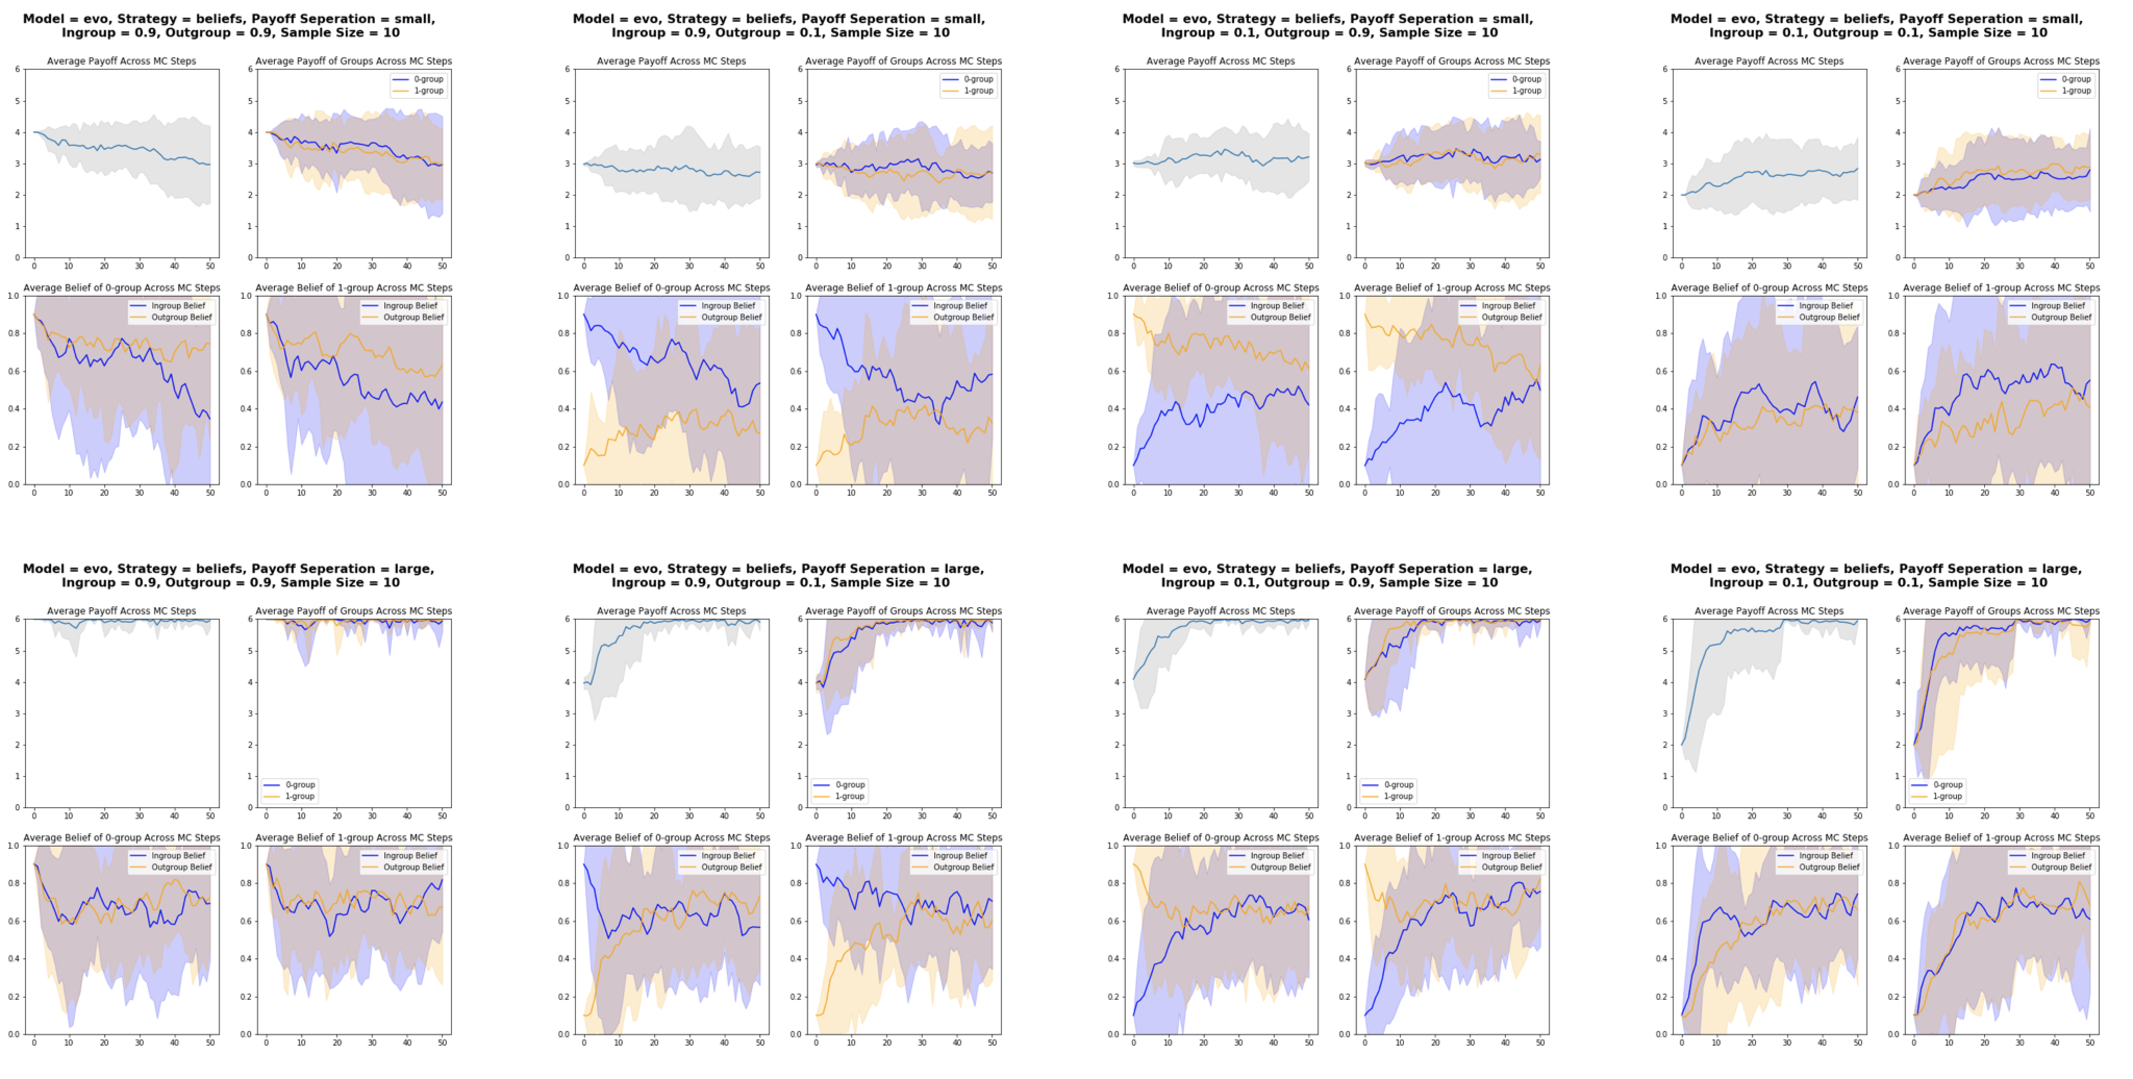
\includegraphics[width=11cm]{images/social_wellmixed1}
\caption{\label{social_wellmixed1} Graphs of the social learning model with the beliefs strategy approach on a well mixed network under every initial belief condition.}
\end{figure}
\begin{figure}
\centering
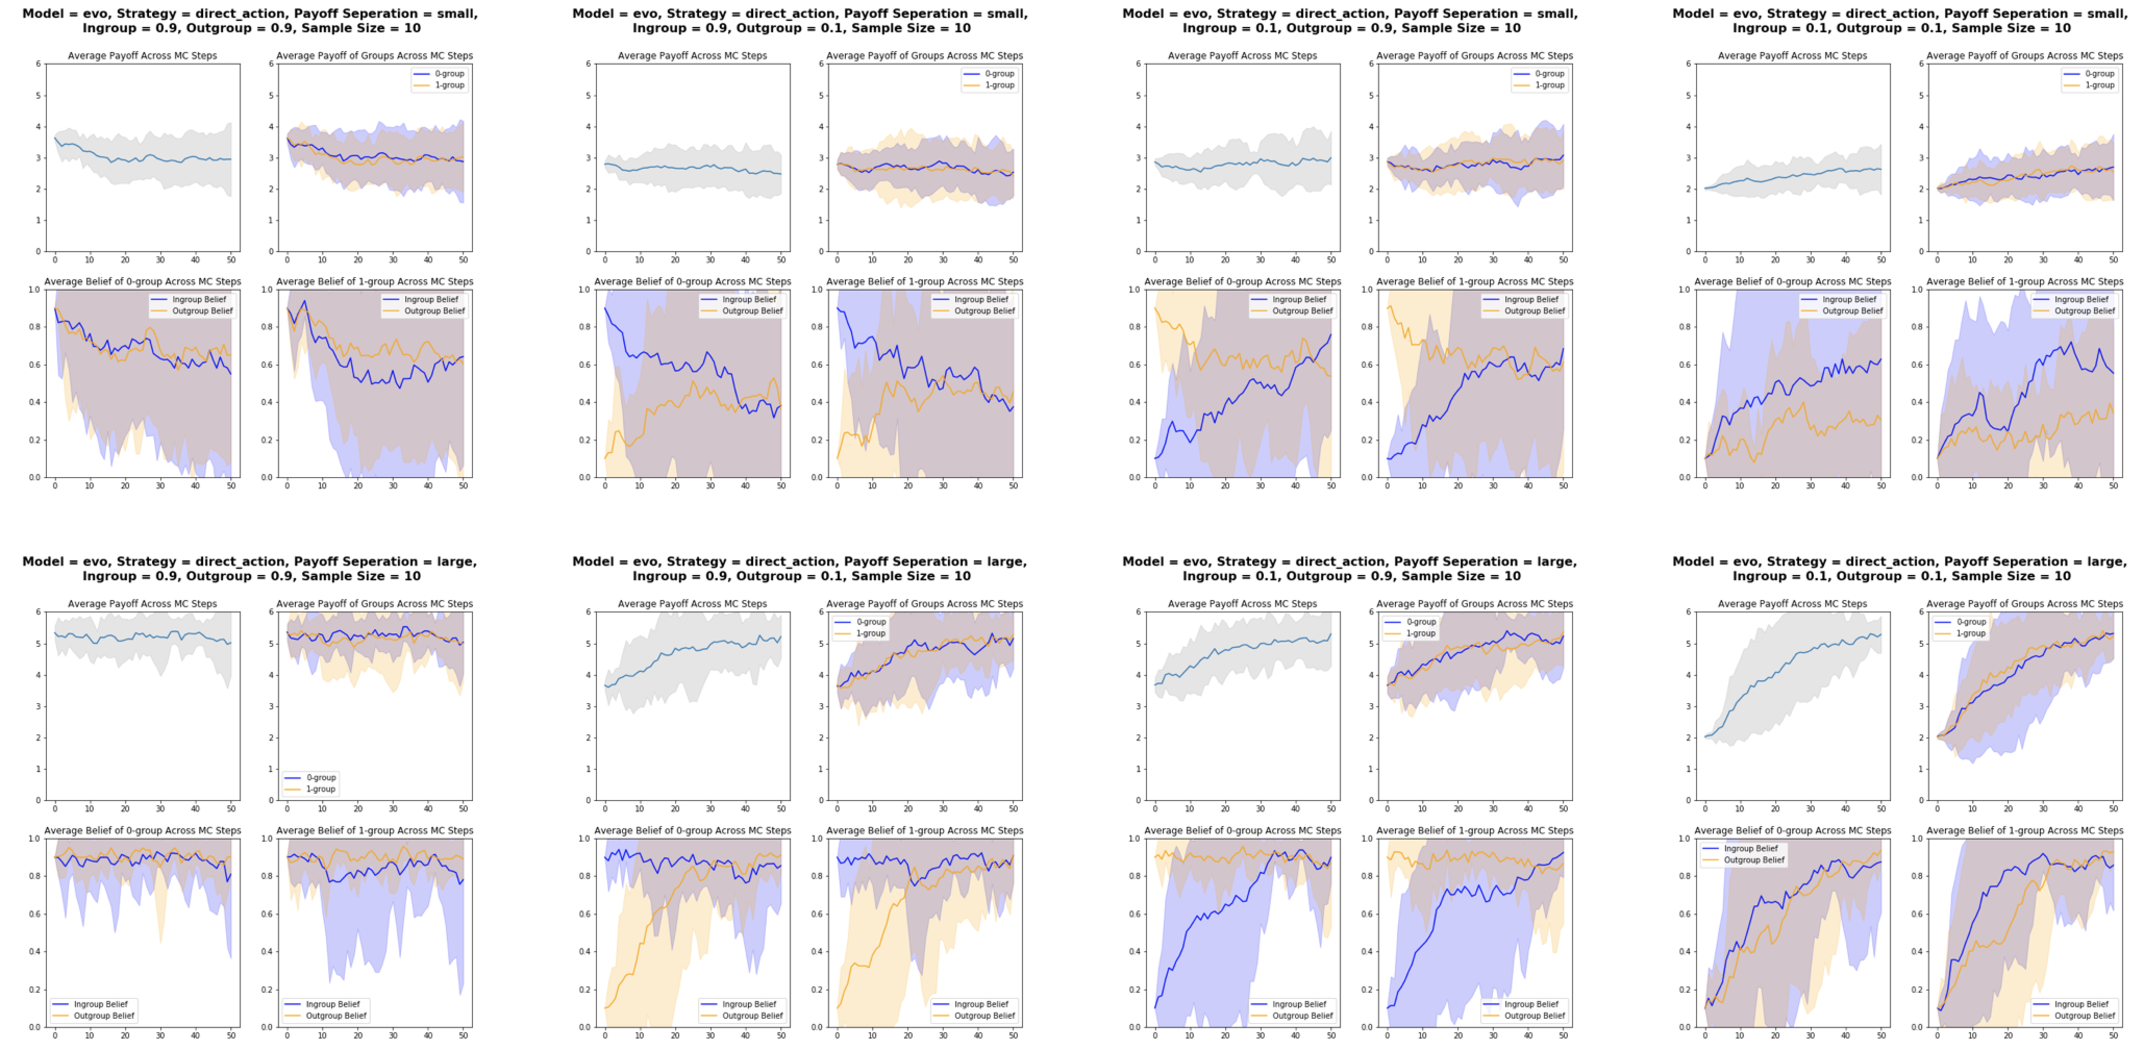
\includegraphics[width=11cm]{images/social_wellmixed2}
\caption{\label{social_wellmixed2} Graphs of the social learning model with the direct actions strategy approach on a well mixed network under every initial belief condition.}
\end{figure}

\subsection{Social learning on a two communities network}
For the beliefs based strategy approach, similar behaviour was observed compared to the well mixed population. For the smaller payoff separation games, beliefs approached middle valued probabilities and initial differences in beliefs diminished. For larger payoff separation games, the beliefs converge to high probabilities and the payoffs quickly converge to the optimal payoff.
However, for the direct actions strategy approach, different behaviour was observed in comparison to the well mixed population. For the small payoff separation games, there was a case when the initial difference in beliefs never diminished and another when a difference in beliefs arose when there wasn’t initially. This could be due to the effect of the divided network structure. Interestly, both of these cases suggest the opposite of prejudice, where agents believe that the opposite group is more likely to cooperate than their own group.
For the games with a large payoff separation and more incentive to cooperate, for all combinations of initial beliefs prejudice arose. In all cases, the ingroup probabilities converge quickly to 1 while the outgroup probabilities are much lower at around 0.7. The payoffs all converged to slightly less than the optimal payoffs.

\begin{figure}
\centering
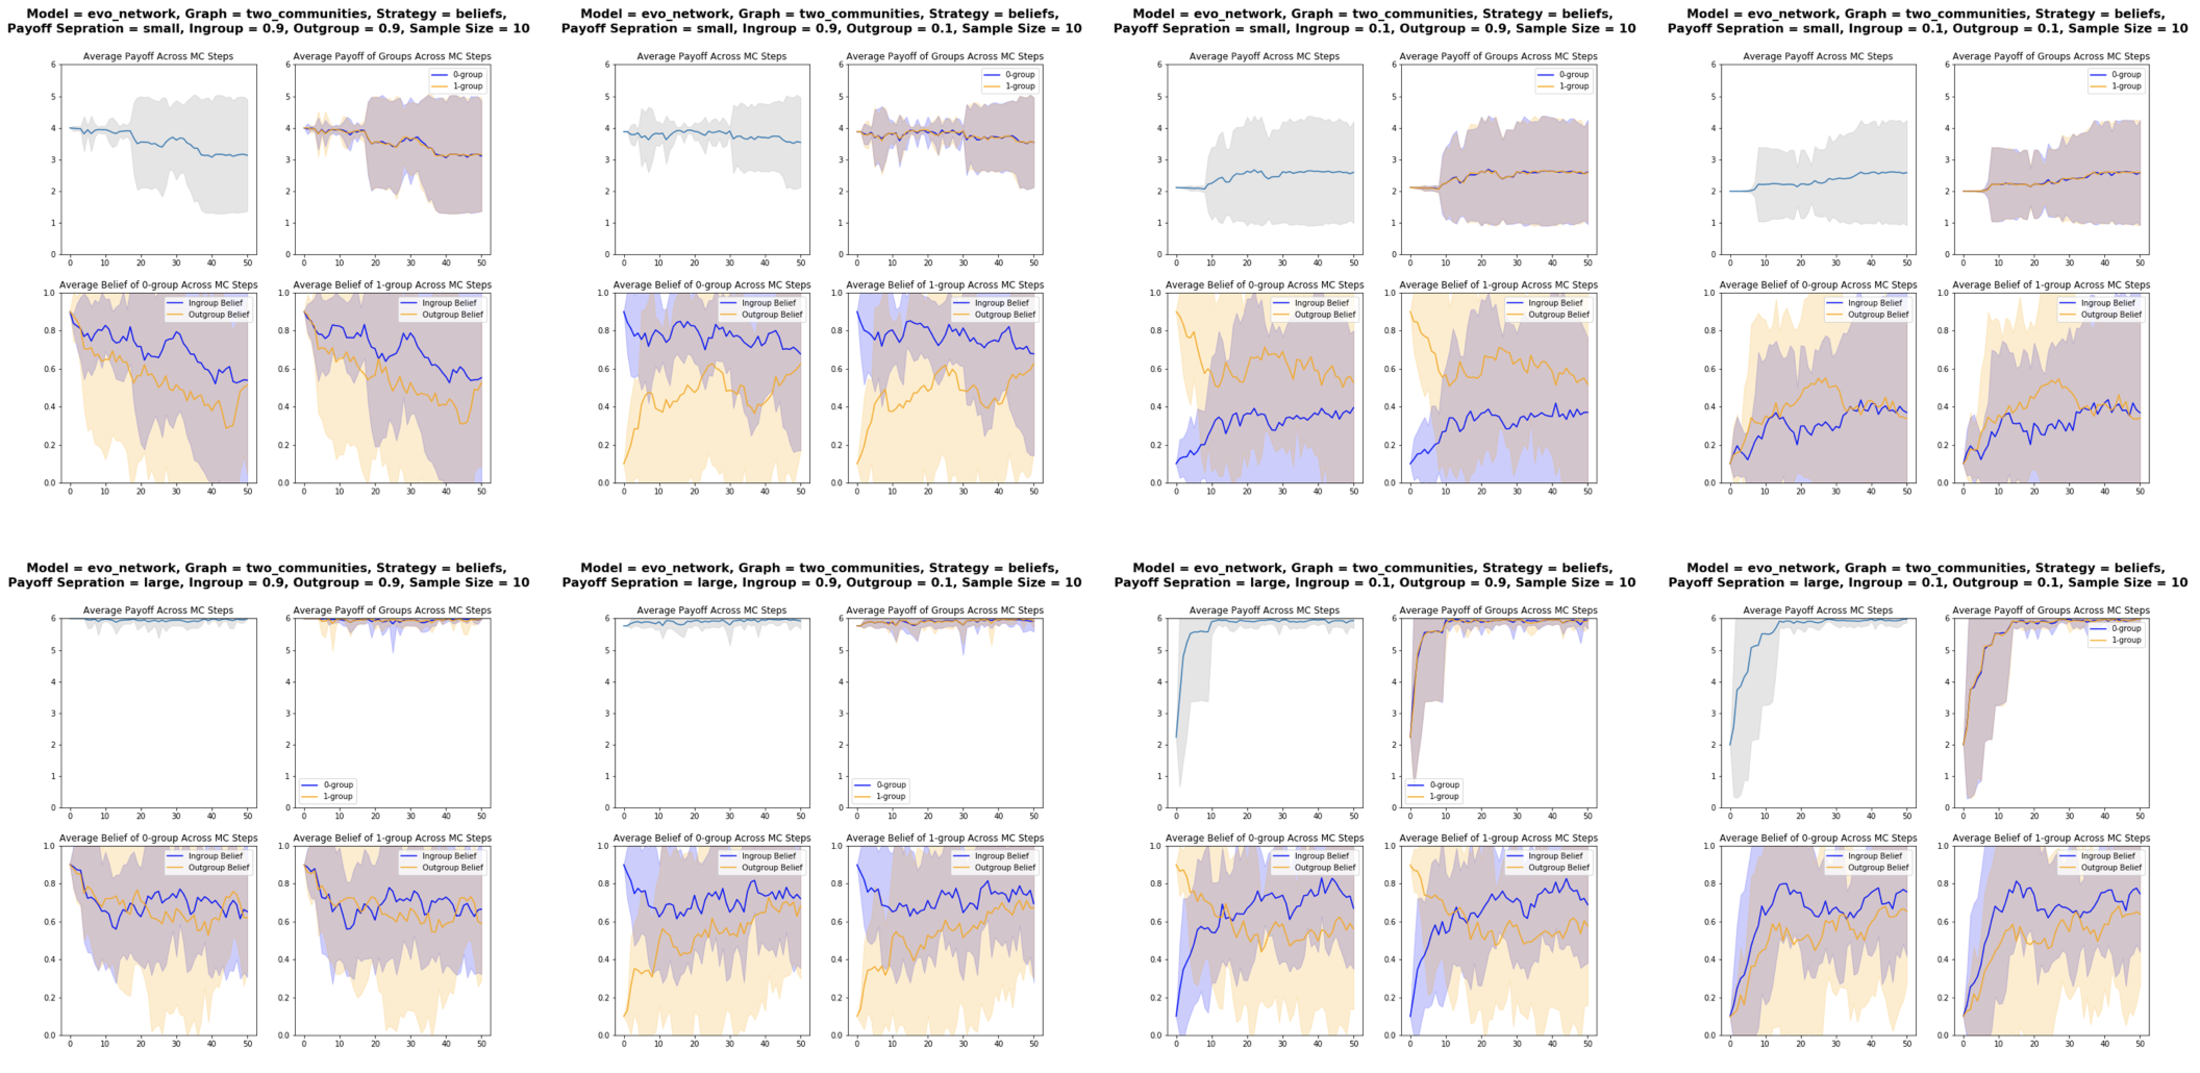
\includegraphics[width=11cm]{images/social_twocommunities1}
\caption{\label{social_twocommunities1} Graphs of the social learning model with the beliefs strategy approach on a two communities network under every initial belief condition.}
\end{figure}
\begin{figure}
\centering
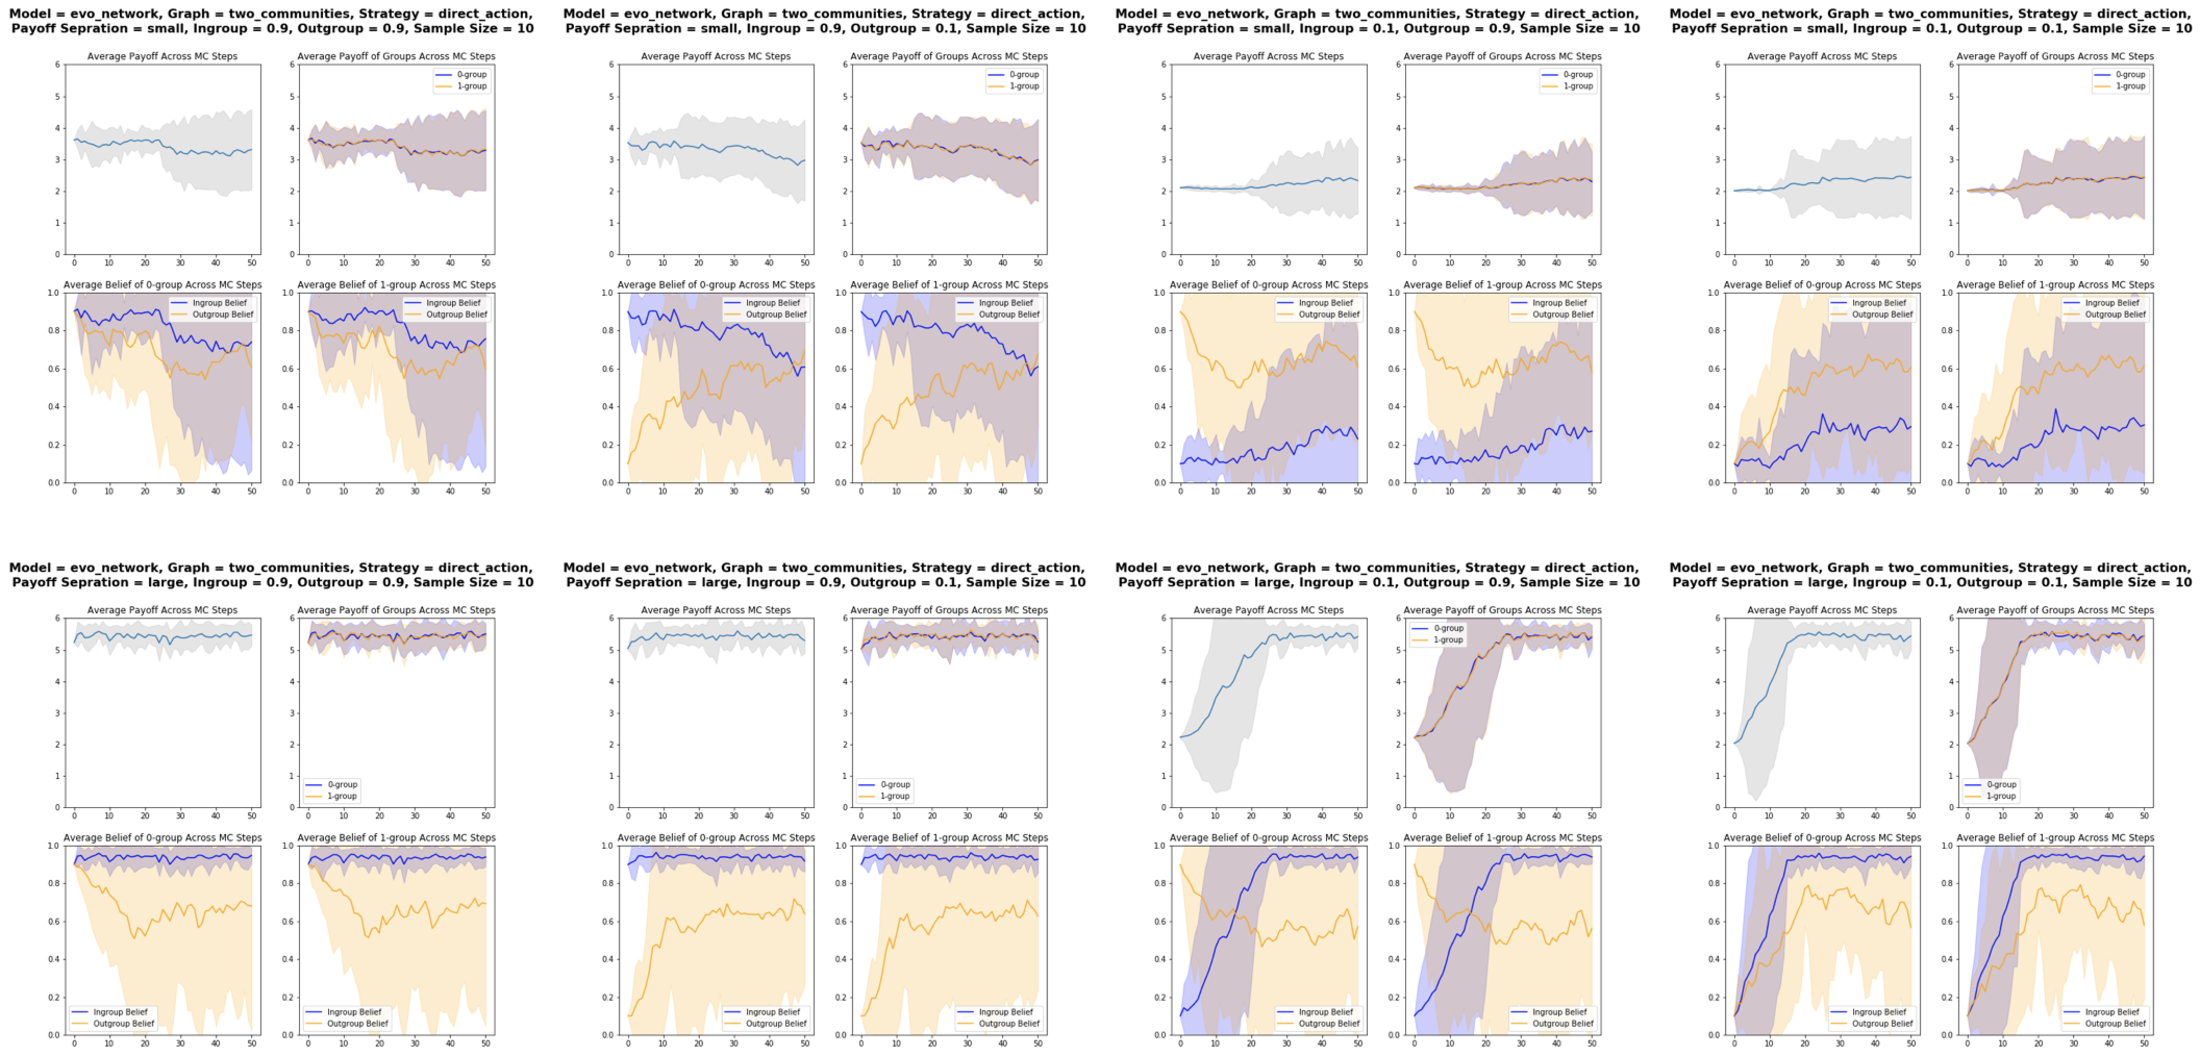
\includegraphics[width=11cm]{images/social_twocommunities2}
\caption{\label{social_twocommunities2} Graphs of the social learning model with the direct actions strategy approach on a two communities network under every initial belief condition.}
\end{figure}

\subsection{Individual learning}
Nearly identical results were observed for individual learning for both network structures, payoff matrices, strategy approaches and initial beliefs. In all cases, the in and outgroup beliefs almost instantly dropped to a value around 0.3 and only very slowly increased over the course of the simulation. In all cases, there is no difference in the in and outgroup beliefs implying the lack of prejudice. Constant payoffs with low variance of around half of the optimal payoffs were achieved in all situations. The results suggest that when all the agents are learning individually, the agents have difficulty learning to cooperate and stick with a defecting strategy, on average. 
To demonstrate the validity of the individual learning (reinforcement learning) method, below are the results from the 2 agent test case. In this model, there is a dummy agent that plays a fixed strategy and a learning agent. The graphs below show the learning agent correctly learning the dummy agent’s fixed strategy of defect and cooperate, respectively, and the Nash equilibriums. Therefore, we are confident in the reinforcement learning algorithm, and suggest that the stagnant results from the 100 agent model is due to the effect of the agents struggling to learn the optimal strategy because every other agent is also changing their strategies in between interactions. 

\begin{figure}
\centering
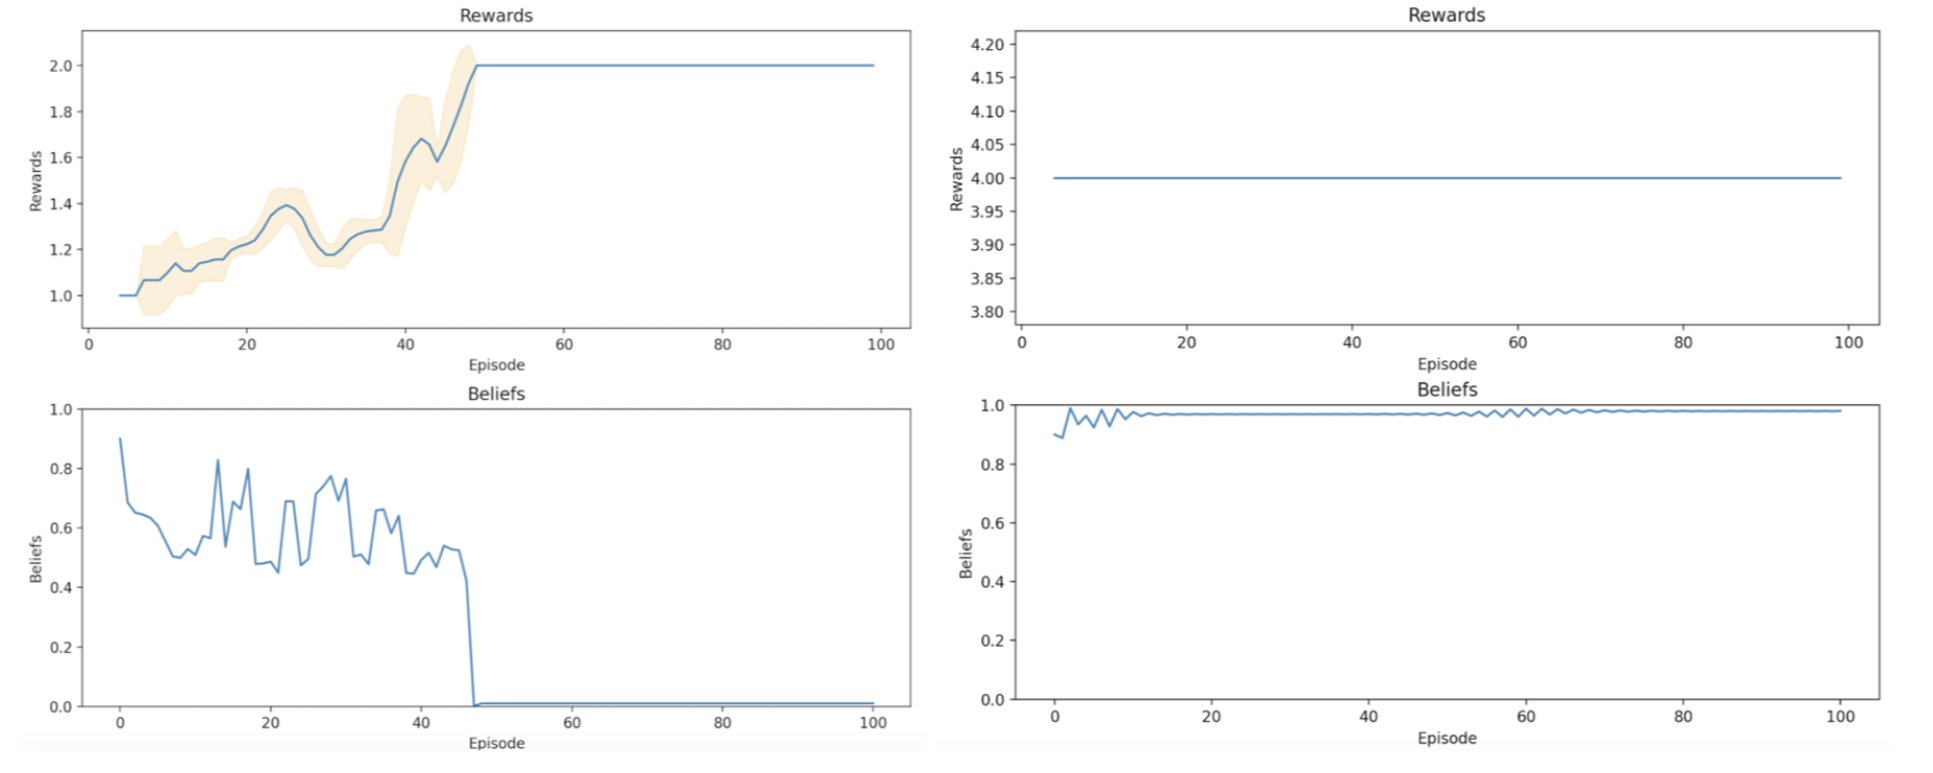
\includegraphics[width=11cm]{images/individual_2agents}
\caption{\label{individual_2agents} Graphs of the individual learning model correctly learning the fixed strategy of a dummy agent.
\end{figure}

\begin{figure}
\centering
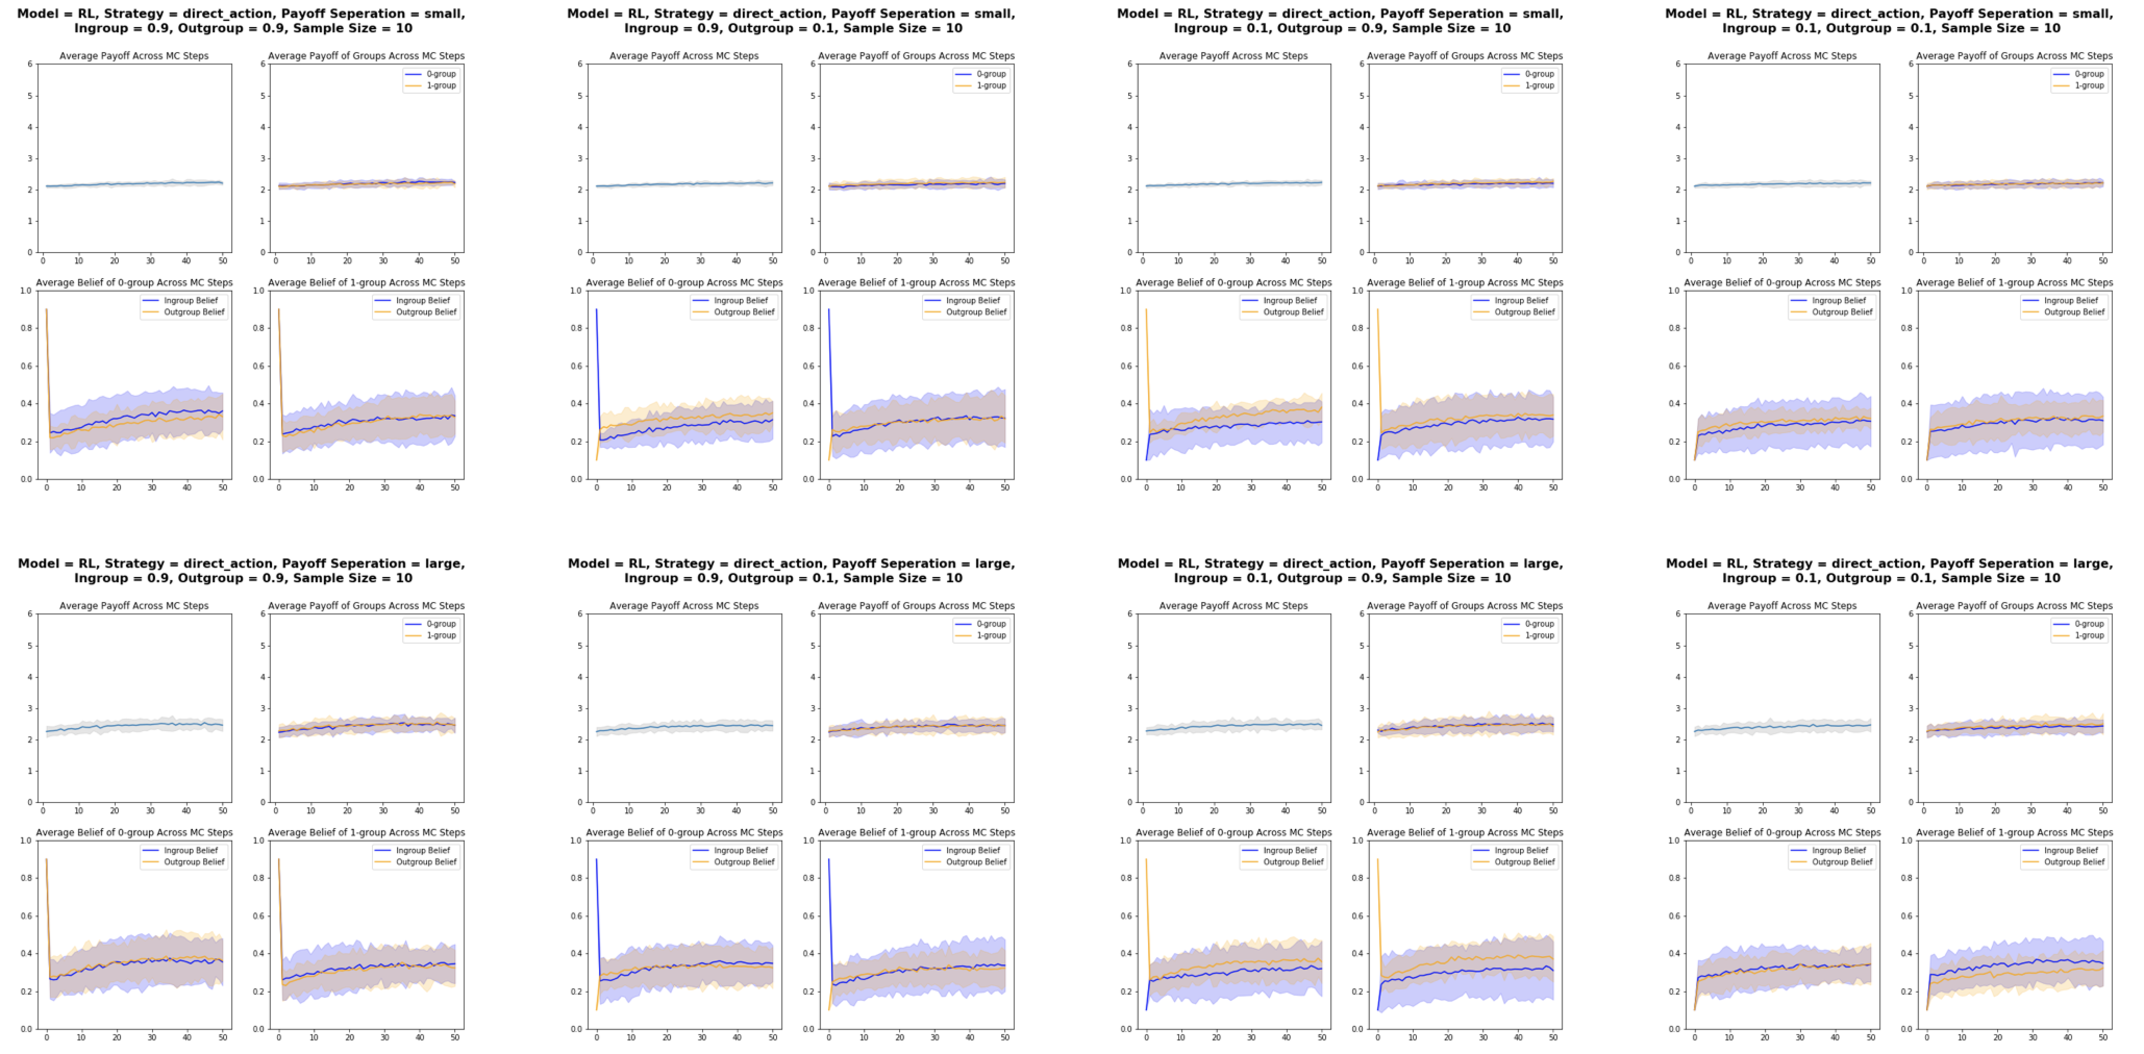
\includegraphics[width=11cm]{images/individual_wellmixed1}
\caption{\label{individual_wellmixed1} Graphs of the individual learning model with the beliefs strategy approach on a well mixed network under every initial belief condition.}
\end{figure}
\begin{figure}
\centering
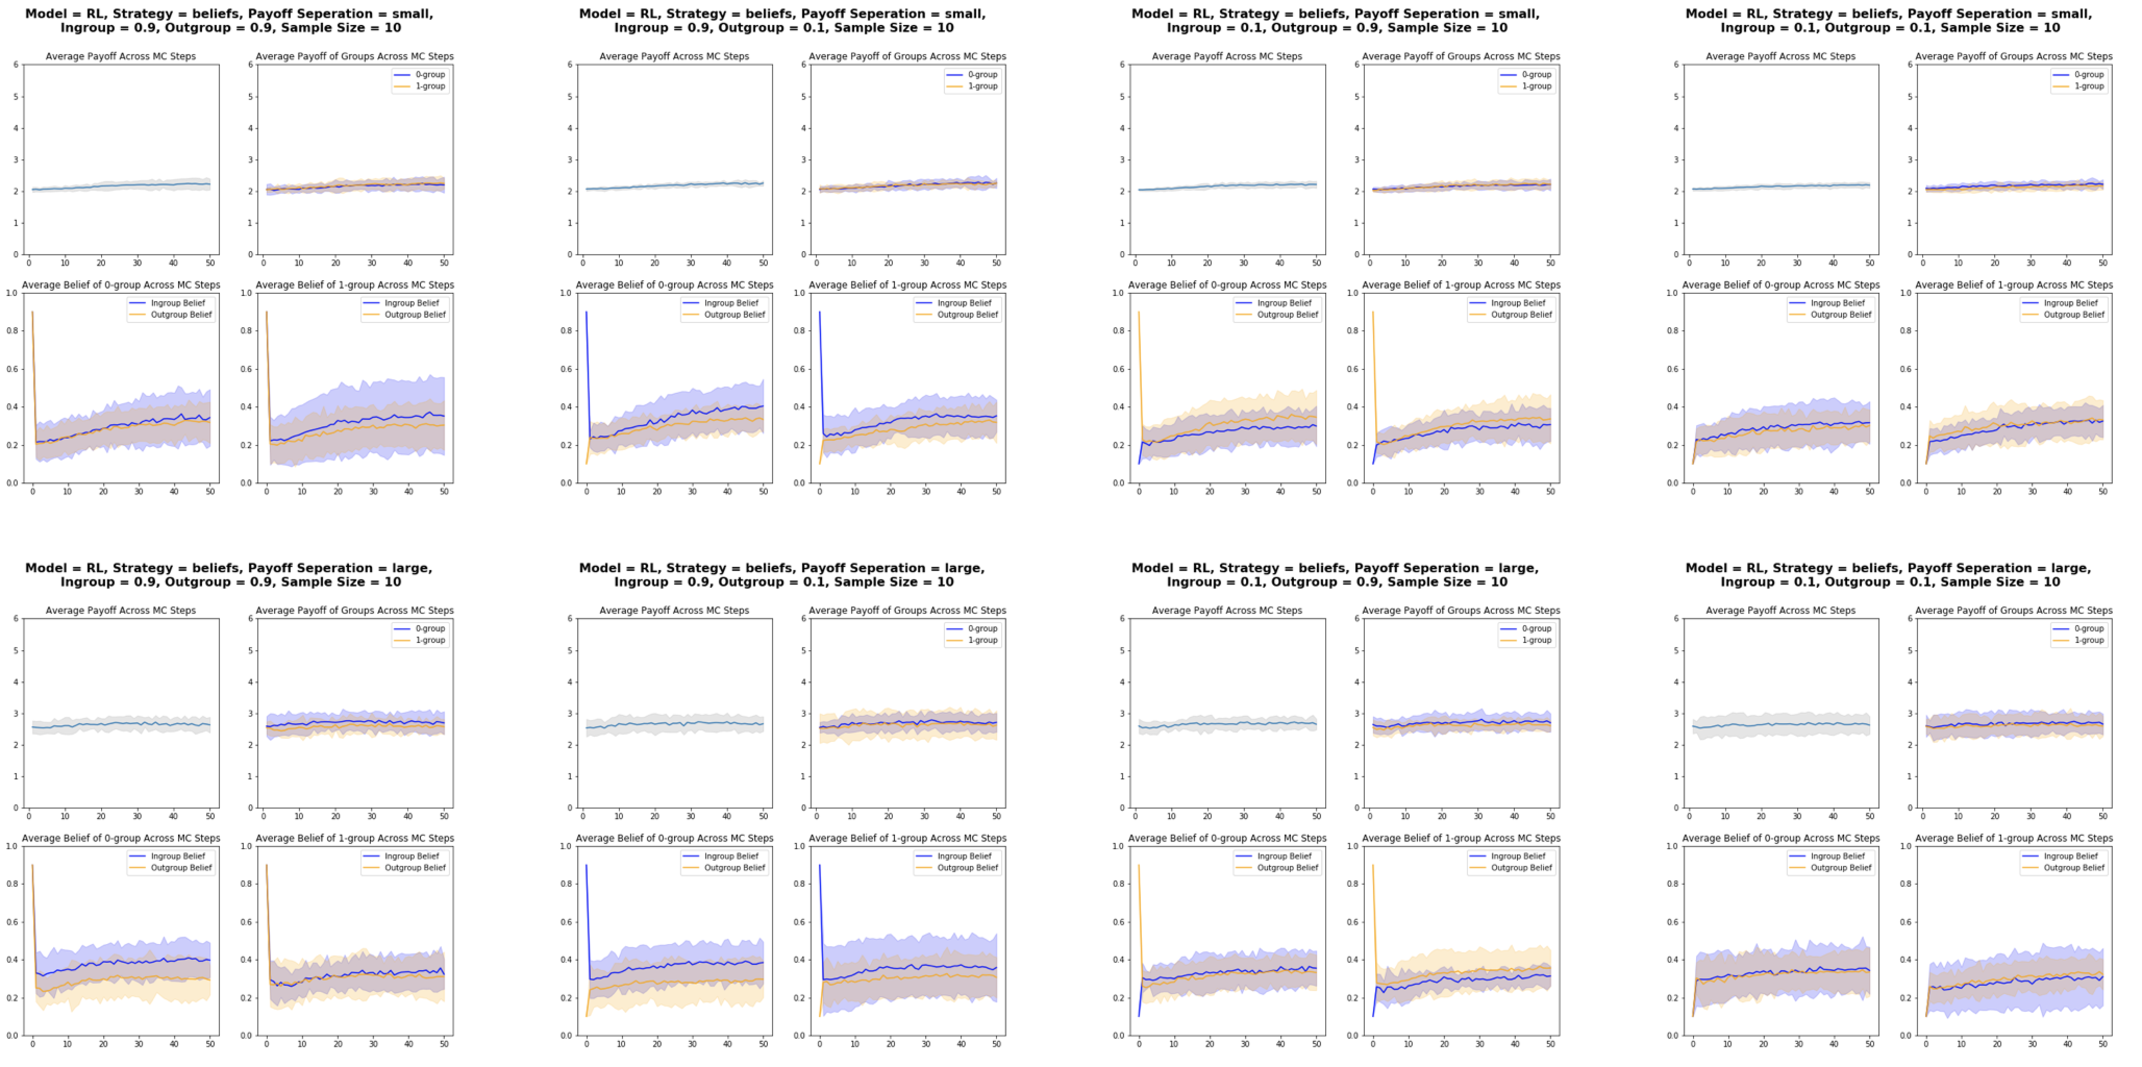
\includegraphics[width=11cm]{images/individual_wellmixed2}
\caption{\label{individual_wellmixed2} Graphs of the individual learning model with the direct actions strategy approach on a well mixed network under every initial belief condition.}
\end{figure}

\begin{figure}
\centering
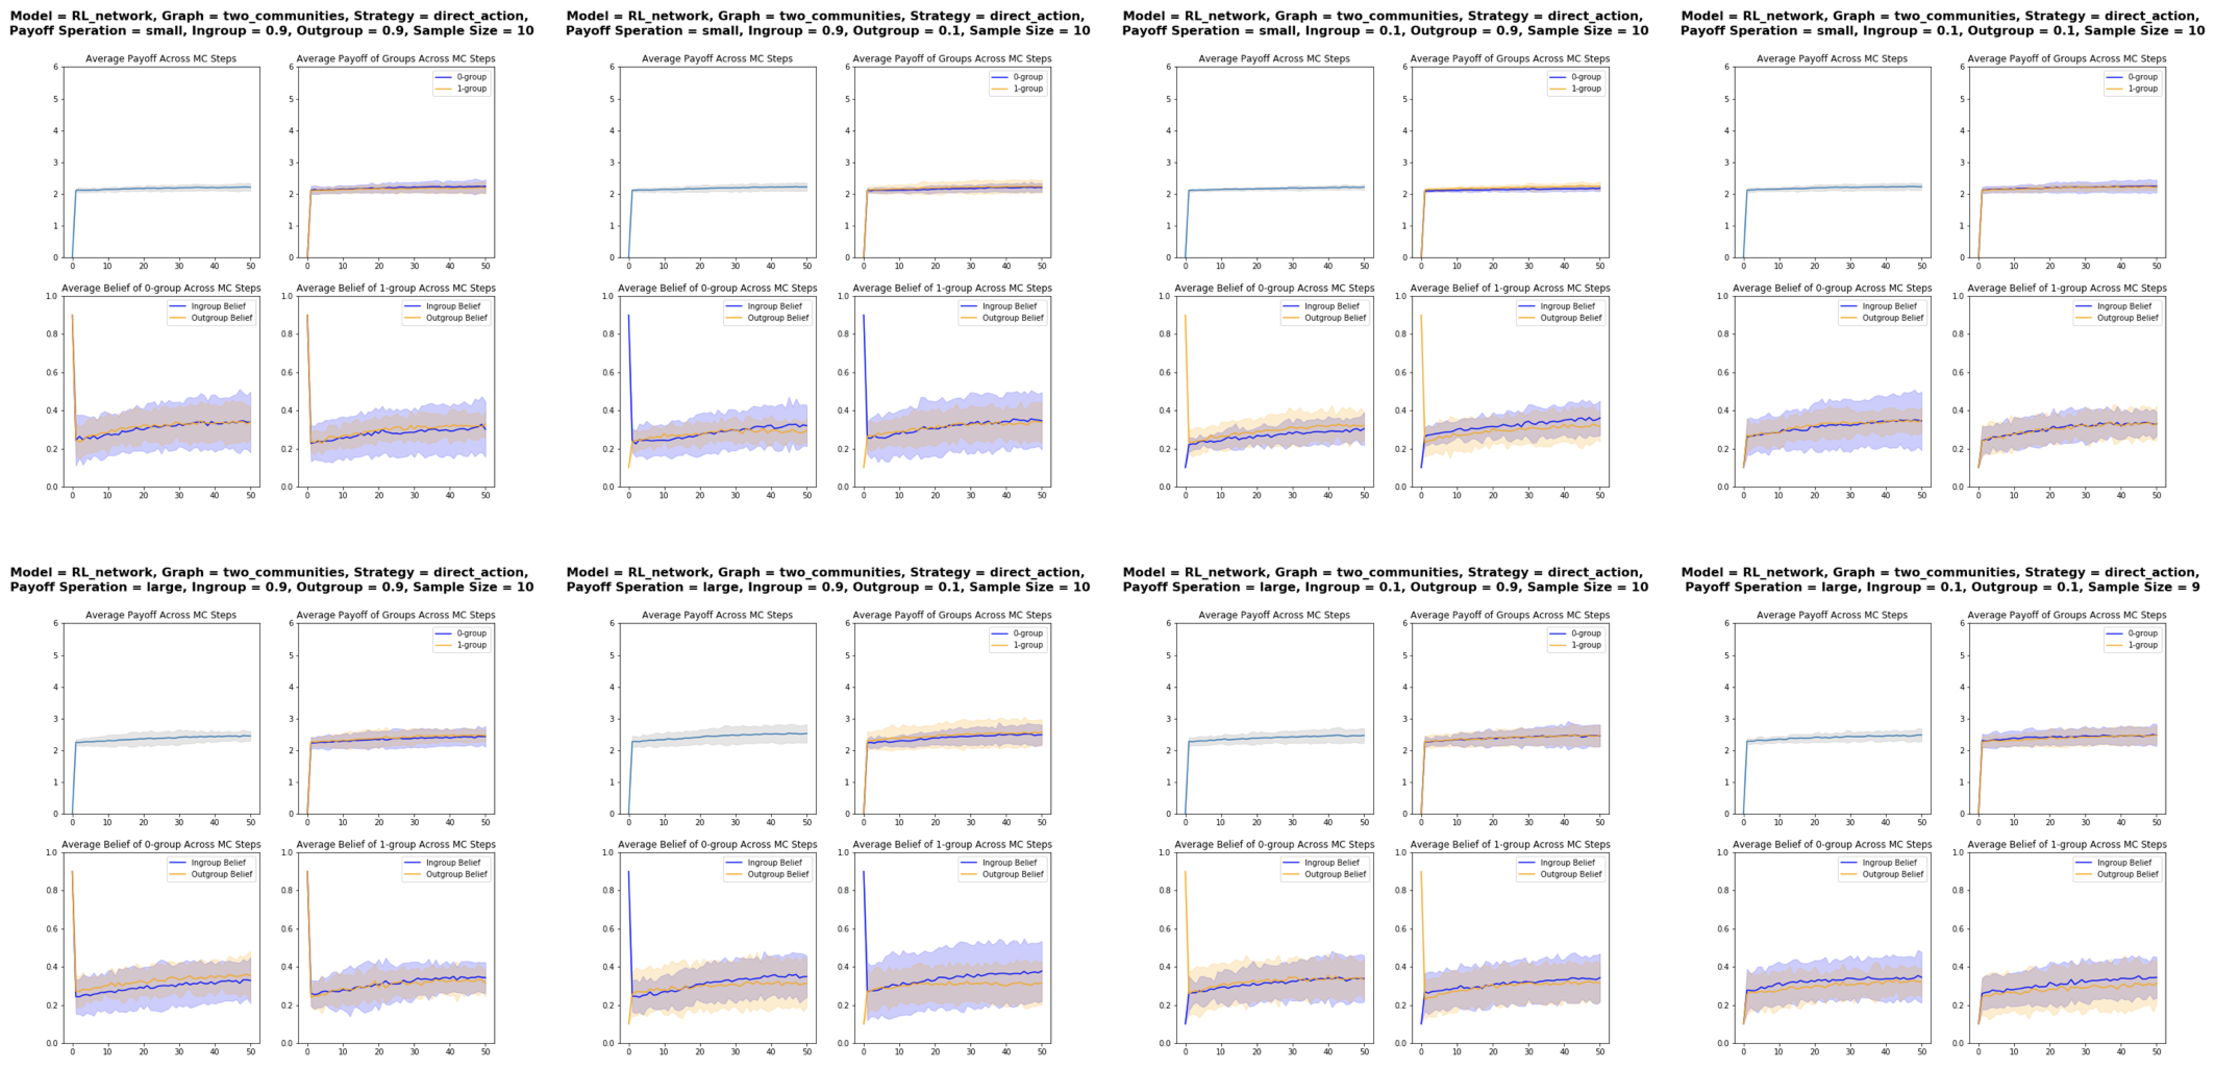
\includegraphics[width=11cm]{images/individual_twocommunities1}
\caption{\label{individual_twocommunities1} Graphs of the individual learning model with the beliefs strategy approach on a two communities network under every initial belief condition.}
\end{figure}
\begin{figure}
\centering
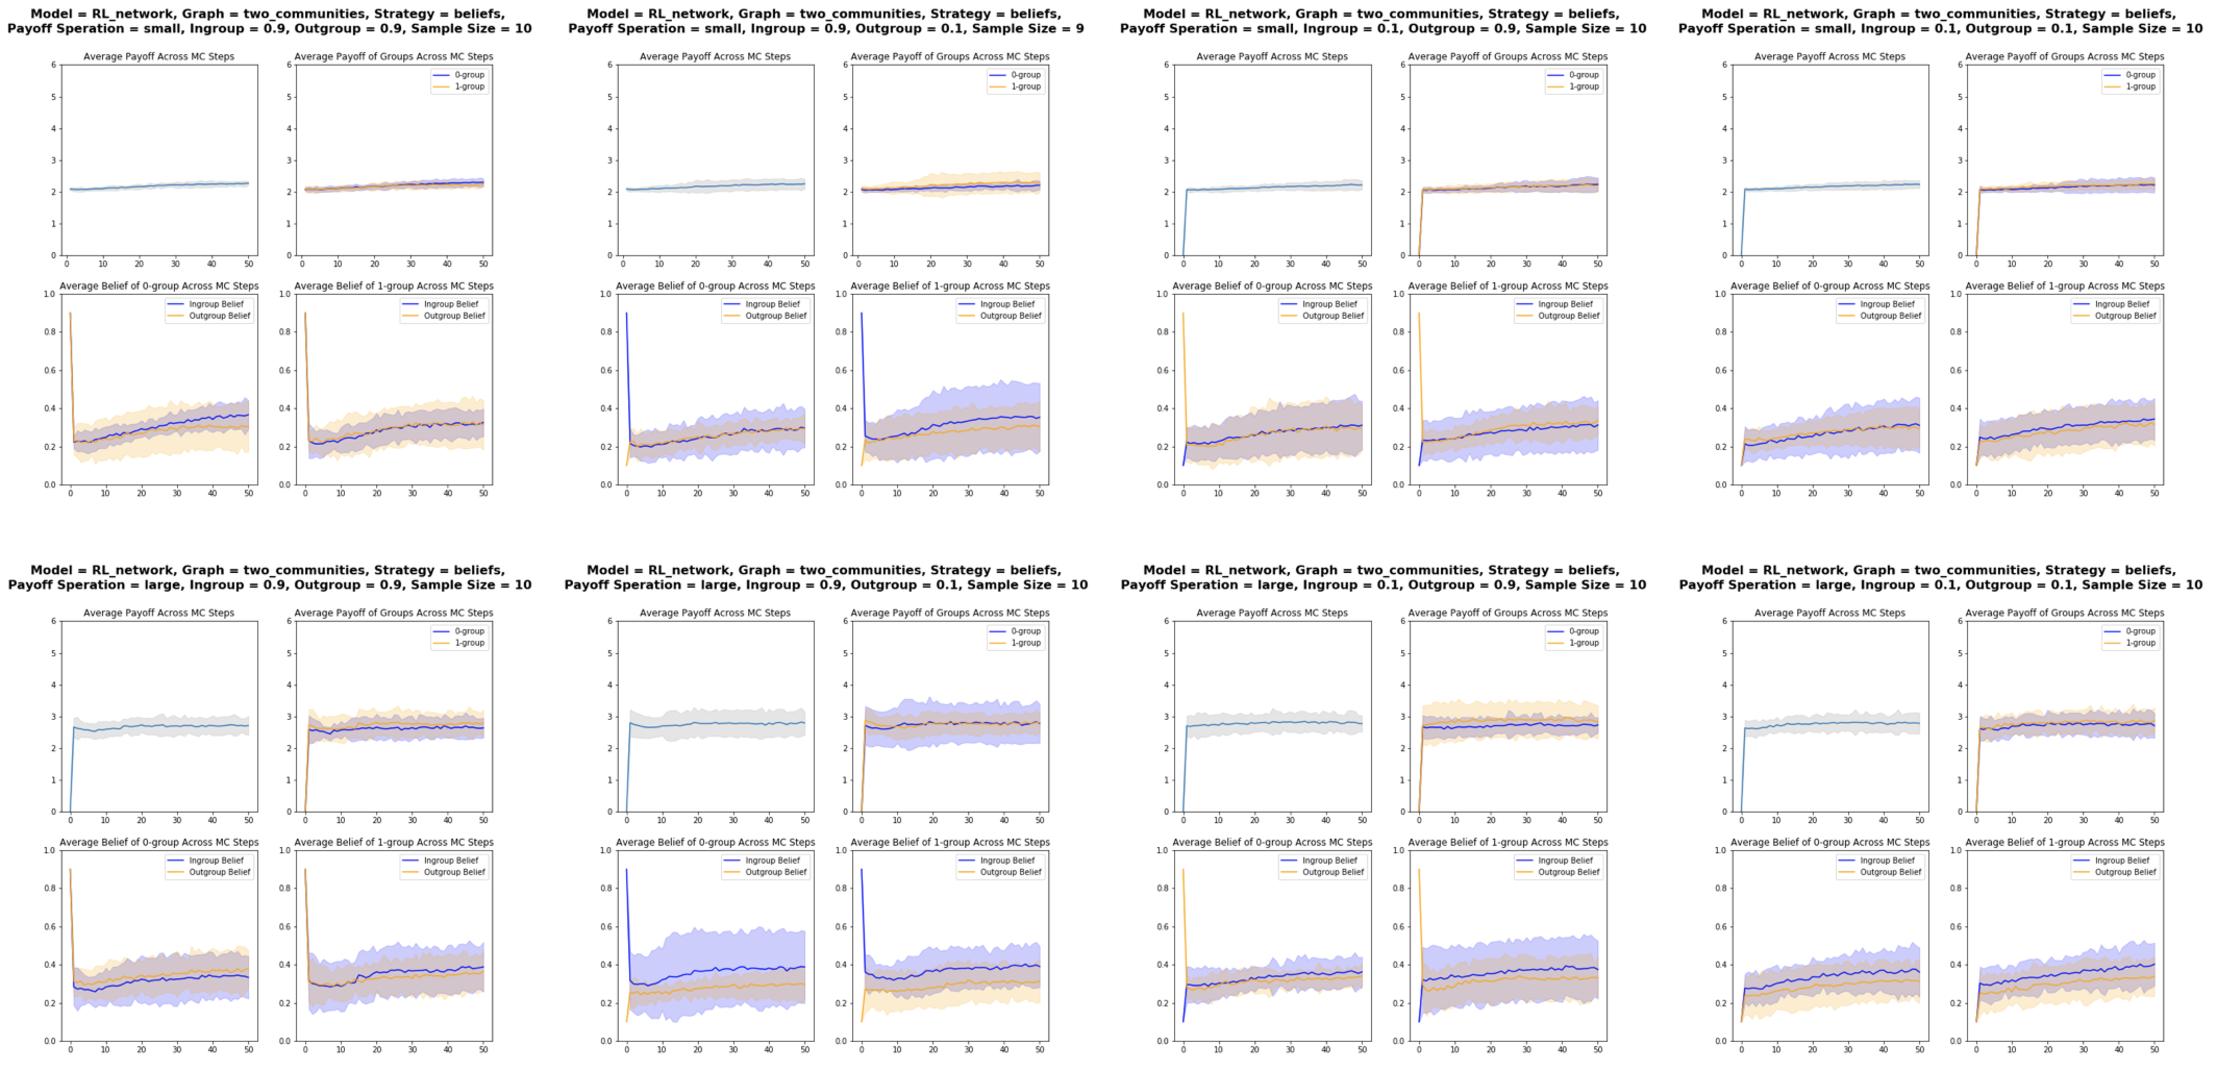
\includegraphics[width=11cm]{images/individual_twocommunities2}
\caption{\label{individual_twocommunities2} Graphs of the individual learning model with the direct actions strategy approach on a two communities network under every initial belief condition.}
\end{figure}
 
\section{Conclusion}
In conclusion, the results suggest that the learning method, social or individual learning, has the greatest effect on the movement of agents’ beliefs.  When the agents learnt strategies as a group from their pooled interactions in the social learning models, the beliefs were able to change over time. Whereas, when individuals updated their beliefs from personal experiences alone, their beliefs fluctuated dramatically less and most agents stuck with a defecting strategy.  The difference in the payoff for cooperating and defecting also had a significant effect on the movement of beliefs for the social learning models. For games with a higher reward for both agents cooperating, agents learnt to cooperate under more initial belief conditions and generally more quickly. The effect of the agents’ choice of strategy was also only observed in the social learning models with the payoffs converging to the optimal payoffs quicker for the beliefs based approach compared to direct actions. Network structure also had an effect on the social learning models, with maximum optimal population payoffs only being able to be achieved in the well mixed population as well as differences in beliefs being more robust to change for the two communities network. 
Finally, prejudice was shown to arise on the two communities network structure, with a direct action strategy approach, a large difference in the payoffs of the Nash equilibrium regardless of the combination of initial beliefs. Directions for future research include investigating the effect of the populations with unequal proportions of group membership and alternative network structures. 


\end{document}
